\documentclass{article}
\usepackage{amsmath}
\usepackage{tikz}
\usetikzlibrary{arrows.meta}

\begin{document}

\begin{figure}[h]
    \centering
    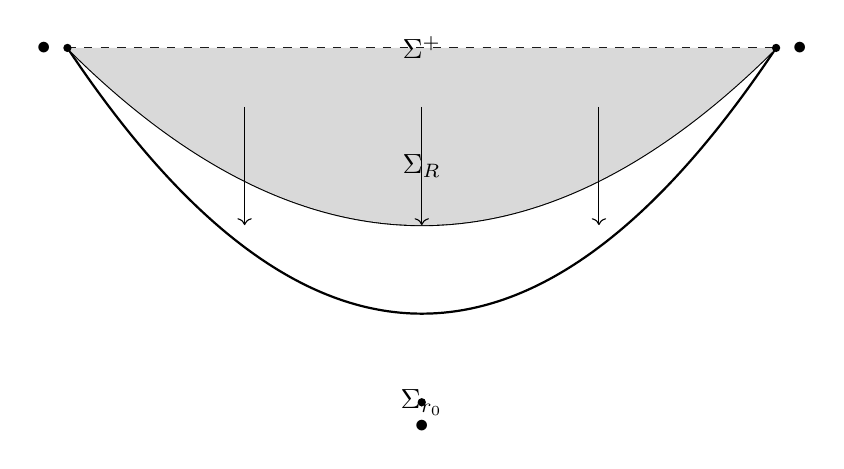
\begin{tikzpicture}[scale=1.5]
        % Draw the outer boundary
        \draw[dashed] (0,0) -- (6,0);
        \draw[thick] (0,0) .. controls (2,-2) and (4,-2) .. (6,0);
        
        % Draw the inner boundary
        \draw[thick] (0,0) .. controls (2,-3) and (4,-3) .. (6,0);
        
        % Fill the region between the boundaries
        \fill[gray!30] (0,0) .. controls (2,-2) and (4,-2) .. (6,0) -- (6,0) -- (0,0);
        
        % Draw the labels
        \node at (3, -1) {$\Sigma_R$};
        \node at (3, 0) {$\Sigma^{+}$};
        \node at (3, -3) {$\Sigma_{r_0}$};
        
        % Draw the vertical lines
        \draw[->] (1.5, -0.5) -- (1.5, -1.5);
        \draw[->] (3, -0.5) -- (3, -1.5);
        \draw[->] (4.5, -0.5) -- (4.5, -1.5);
        
        % Draw the points
        \fill (0,0) circle (1pt);
        \fill (6,0) circle (1pt);
        \fill (3,-3) circle (1pt);
        
        % Label the points
        \node at (-0.2, 0) {$\bullet$};
        \node at (6.2, 0) {$\bullet$};
        \node at (3, -3.2) {$\bullet$};
    \end{tikzpicture}
    \caption{Spacetime region on which we solve the wave equation on the interior of the expanding region. We solve a sequence of finite problems, i.e., we consider a solution $\psi_R$ with prescribed data on $\Sigma_R$, and then show that the limit $\lim_{R \to \infty} \psi_R$ exists in a suitable energy space. In this step, we solve up to a $\Sigma_{r_0}$ hypersurface, where $r_0 > r_{\mathcal{C}}$.}
    \label{fig:wave_equation_region}
\end{figure}

\end{document}